\section{Fast Coresets in Practice}

Despite the near-linear time algorithm described in Sections~\ref{sec:theory} and~\ref{sec:logdelta}, the coreset construction in \ref{alg:main} nonetheless
requires an $O(1)$ approximation to the original task before the sampling can occur. Although theoretically justified, it is unclear how necessary this is in
practice -- would a worse approximation factor still be representative of the dataset for for practical purposes? We answer this question by defining a suite of
algorithms, datasets and evaluation procedures that allow for a comprehensive study of speed vs. accuracy tradeoffs in compression for clustering.  We begin by
describing our experimental setup before showing results in both the static and streaming settings.  Lastly, we highlight how this corresponds to downstream
clustering tasks.

\subsection{Experimental Setup}
\subsubsection{Metrics}
\label{sssec:metrics}

We analyze the sampling methods along two metrics -- compression accuracy and construction time. Although measuring runtime is standard, predicting coreset
quality is a more difficult task. Specifically, it is unclear how to confirm that a subset of points satisfies the coreset property over all solutions. To this
end, we use the following distortion measure introduced in~\cite{chrisESA} \[ \max \left( \dfrac{\cost(P, \calC_{S})}{\cost(S, \calC_{S})}, \dfrac{\cost(S,
\calC_{S})}{\cost(P, \calC_{S})} \right),\] where $\calC_{S}$ is a candidate solution that was computed over the coreset $S$. This
will be within $1+\varepsilon$ if the coreset guarantee is satisfied but may be unbounded otherwise.  We refer to this metric as the \emph{coreset distortion}.
For completeness, we also measure the absolute cost incurred by $calC_S$ on the original dataset.

\subsubsection{Algorithms}
\label{ssec:algorithms}

We compare our method (Algorithm~\ref{alg:main}) against 4 different benchmark sampling strategies that span the space between optimal sublinear time and
optimal accuracy guarantees.
\begin{itemize}
        \item \emph{Standard uniform sampling}. Weights are all equal to $n / m$, where $m$ is the size of the sample.
        \item \emph{Lightweight coresets \cite{bachem2018scalable}}. Lightweight coresets find the mean $\mu$ of the dataset and obtain per-point sensitivity estimates by $\hat{s}(p) = 1/|P| + \cost(p, \mu) / \cost(P, \mu)$. The goodness of this algorithm depends on how well these scores approximate \cref{eq:sensitivity}.
        \item \emph{Standard sensitivity sampling \cite{LS10}}. We follow the standard approach for sensitivity sampling outlined in Section~\ref{ssec:sens_sampling}.
        \item \emph{Welterweight coresets}: This is a generalized interpolation between lightweight coresets and the `heavy-duty' sensitivity sampling coresets. For any $j
            \in \{1,..., k\}$, we compute a coreset using sensitivity sampling with respect to a candidate $j$-means++ solution.
\end{itemize}

We take a moment here to motivate the welterweight coreset algorithm.  Consider that lightweight coresets are simply solving $1$-means to obtain sensitivity
values whereas sensitivity sampling is solving the $k$-means problem. Given that sensitivity values are estimated via $ \sigma_\calC(p) = \dfrac{\cost(p,
\calC)}{\cost(\calC_{p}, \calC)} + \dfrac{1}{|\calC_p|},$ changing the value of $j$ affects the cluster sizes $|\calC_p|$ and therefore acts as a direct
interpolation between uniform and sensitivity sampling.  We analyze the different choices of $j$ in Table~\ref{tbl:class-imbalance} and default to $j = \log k$
in the other experiments.

\subsubsection{Datasets}
\label{sssec:datasets}

We employ several real and artificial datasets to evaluate the quality of a coreset.  For our real-world data, we utilize the Adult~\cite{Dua:2019},
MNIST~\cite{mnist}, Song~\cite{song}, Census~\cite{census}, and Cover Type~\cite{covtype} datasets, whose characteristics are summarized in
Table~\ref{tbl:datasets} below. These are standard datasets for coreset and clustering evaluations.

\begin{table}[htbp]
    \centering
    \begin{tabular}{lrr}
        Dataset & Points & Dim \\
        \hline
        \emph{Adult} & 48\,842 & 14 \\
        \emph{MNIST} & 60\,000 & 784 \\
        \emph{Song} & 515\,345 & 90 \\
        \emph{Cover Type} & 581\,012 & 54 \\
        \emph{Census} & 2\,458\,285 & 68 \\
        \hline
        \vspace*{0.1cm}
    \end{tabular}
    \caption{Description of real world datasets}
    \label{tbl:datasets}
\end{table}

To complement those, we use several artificial datasets to highlight specific settings. Unless stated otherwise, $n = 50\,000$ and $d=50$.
\begin{itemize}

    \item \emph{c-outlier}. Place $n-c$ points in a single location and $c$ points placed at a large distance away.

    \item \emph{Geometric}. Place $c k$ points at $(1, 0, 0, \cdots)$, $\frac{ck}{r}$ points at $(0, 1, 0, \cdots)$, $\frac{ck}{r^2}$ points
        at $(0, 0, 1, \cdots)$, and so on for $\log_r (ck)$ rounds. Thus, the data creates a high-dimensional simplex with uneven weights across the vertices. We
        default to $c = 100$ and $r=2$.

    \item \emph{Gaussian mixture}. A set of scattered Gaussian clusters of varying density. These clusters are sequentially defined, with the size of the first
        cluster defined by $\frac{n}{\kappa} \exp \left( \gamma \rho_0 \right)$, where $\kappa$ is the number of Gaussian clusters, $\rho_0$ is
        uniformly chosen from $[-0.5, 0.5]$, and $\gamma$ is a hyperparameter that affects the distribution of cluster sizes. 
        Then, given clusters $\{c_1, \cdots, c_i\}$, we obtain the size of the $(i+1)$-st cluster by 
        \[|c_{i+1}| = \frac{n - \sum_i |c_i|}{\kappa - i}\exp \left( \gamma \rho_{i+1} \right).\]
        This has the property $\gamma = 0$ gives only clusters of size $n / k$ and, as $\gamma$ grows, the cluster sizes diverge in size at an exponential rate.
        We note that this is a well-clusterable instance with respect to cost stability conditions, see \cite{AwS12,Cohen-AddadS17,KuK10,ORSS12}.

    \item \emph{Benchmark}. A specific distribution of points introduced in \cite{chrisESA} as a good testbed for coreset algorithms.  It has the property that
        all reasonable $k$-means solutions are of equal quality but are maximally far apart in the solution space. Thus, the dataset is fully determined by the
        number of centers $k$. We follow the advice in the benchmark's original presentation and produce three benchmark datasets of varying size before
        applying random offsets to each. We choose the sizes by $k_1 = \frac{k}{c_1}$, $k_2 = \frac{k - k_1}{c_2}$, and $k_3 = k - k_1 - k_2$ for $c_1, c_2 \in
        \mathbb{R}^+$.

\end{itemize}

Each artificial dataset is constructed to test for a particular set of characteristics. For example, the $c$-outlier problem contains very little information
and, as such, should be simple for any sampling strategy that builds a reasonable representation of its input. The geometric dataset then increases the
difficulty by having $\log k$ clusters and, subsequently, more regions of interest that must be sampled. The Gaussian mixture dataset is harder still, as it
incorporates uneven inter-cluster distances and inconsistent cluster sizes. Lastly, the benchmark dataset is devised to be a worst-case example for sensitivity
sampling.

In all real and artificial datasets, we add random uniform noise $\eta$ with $0 \leq \eta_i \leq 0.001$ in each dimension in order to make all points unique.
Unless specifically varying these parameters, we default all algorithms in~\ref{ssec:algorithms} to $k=100$ for the Adult, MNIST, and artificial datasets and
$k=500$ for the Song, Cover Type, and Census datasets. Our default coreset size is then $m = 40k$. We refer to the coreset size scalar as the \emph{$m$-scalar}.
We only run the dimension-reduction step on the MNIST dataset, as the remaining datasets already have sufficiently low dimensionality. We run our experiments on
an Intel Core i9 10940X 3.3GHz 14-Core processor without parallelization.

\subsection{Evaluating Sampling Strategies}
\label{ssec:alg_qualities}

\paragraph*{Theoretically guaranteed methods.}

\begin{figure*}
\label{fig:coreset_size_on_sens_quality}
\centering
\begin{tabular}{lc}
    \rotatebox[origin=l]{90}{\bf \;\quad\quad\quad\quad\quad\quad\quad$k$-Median} &
    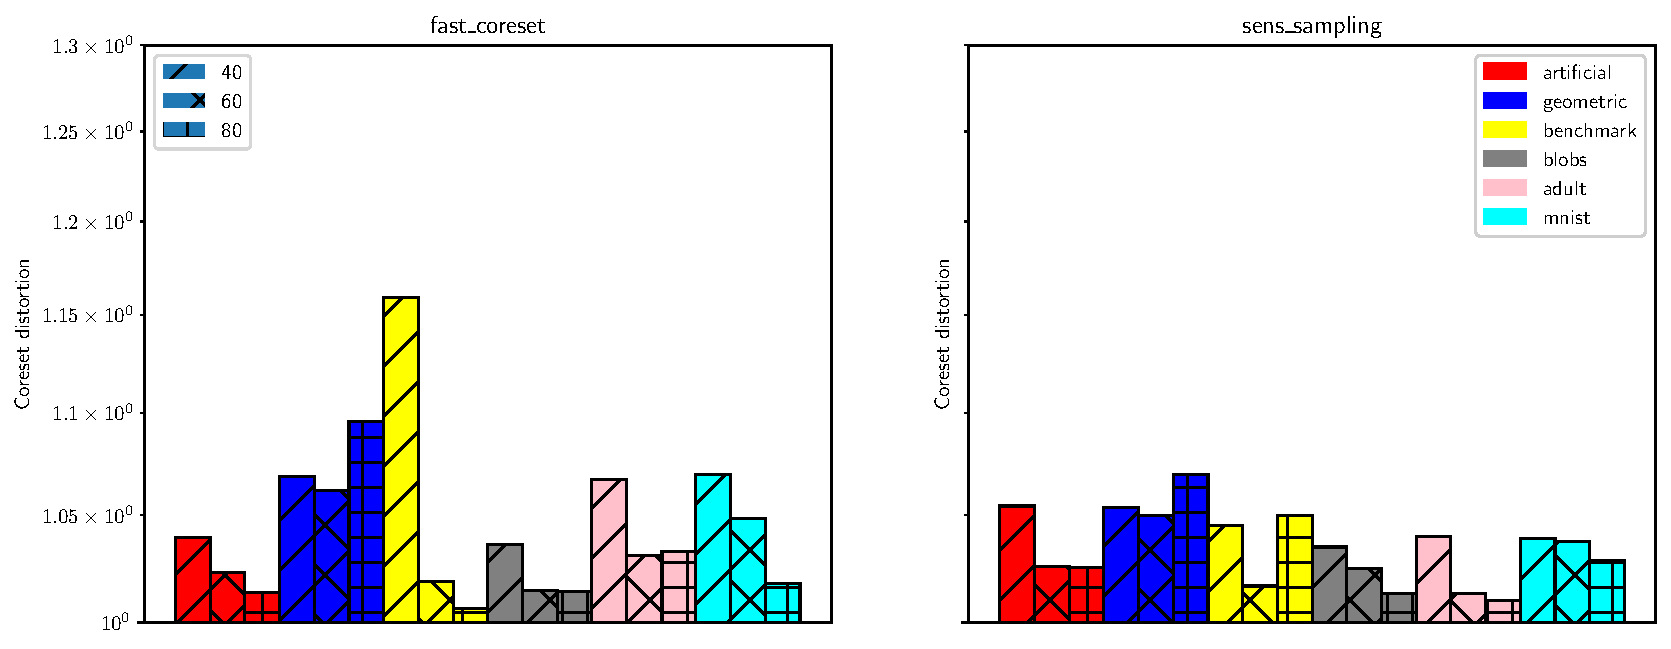
\includegraphics[width=.95\linewidth]{images/1/coreset_distortion-m_scalar_for_sens_sampling.pdf} \\

    \rotatebox[origin=l]{90}{\bf \;\;\quad\quad\quad\quad\quad\quad\quad$k$-Means} &
    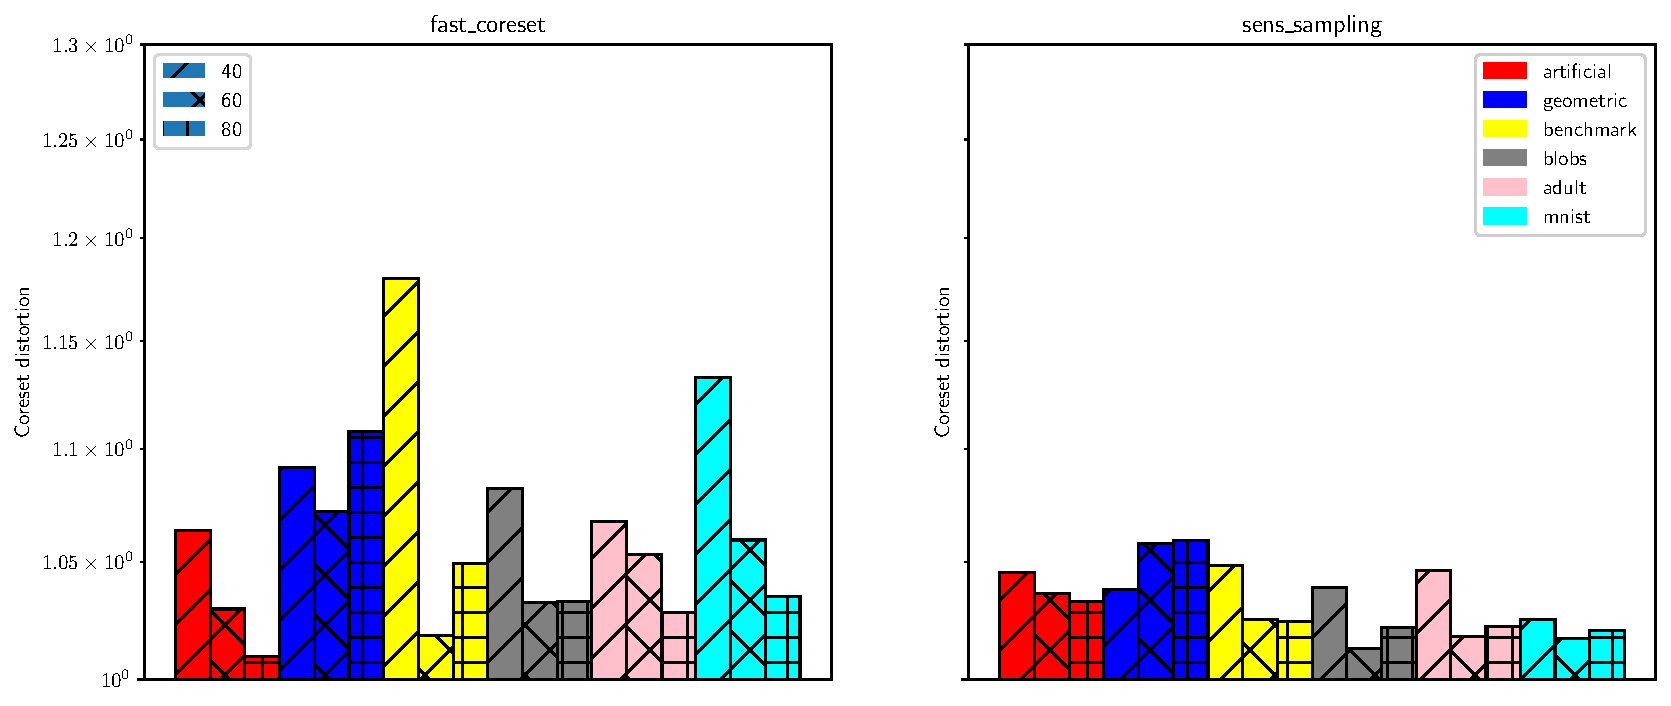
\includegraphics[width=.95\linewidth]{images/2/coreset_distortion-m_scalar_for_sens_sampling.pdf}
\end{tabular}
\caption{The effect of the coreset size on the distortion metric for sensitivity sampling approaches.
We point out that all distortion values are well below $\varepsilon = 0.2$.
Thus, for sufficient coreset sizes, there does not seem to be a meaningful difference between using Fast-Kmeans++ vs. regular Kmeans++.}
\end{figure*}


We first compare the Fast-Coreset algorithm with standard sensitivity sampling to ensure that it obtains comparable accuracy in a smaller runtime.  To this end,
the top of Figure~\ref{fig:coreset_size_on_sens_quality} shows that, across datasets and values of the $m$-scalar, the Fast-Coreset method produces coresets of
quality consistent with traditional sensitivity sampling. Furthermore, choosing a sufficient coreset size ($m$-scalar$=80$) gives distortion below $1.05$ for
both Fast-Coresets and traditional sensitivity sampling. Despite this, we see in the bottom of Figure~\ref{fig:coreset_size_on_sens_quality} that varying $k$
from $50$ to $400$ causes a linear slowdown in sensitivity sampling but only a logarithmic one for the Fast-Coreset method.

This analysis confirms the theory predicted in Section~\ref{sec:theory}: Fast-Coresets run with little overhead while retaining the accuracy of sensitivity sampling.
Given this context, we do not add traditional sensitivity sampling to further experiments, as it is infeasible to run on large datasets.

\paragraph*{Speed vs. Accuracy.}

We now refer the reader to Figure~\ref{fig:coreset_size_on_quality}, where we show the effect of coreset size across the real-world datasets by sweeping over
$m$-scalar values. Despite the suboptimal theoretical guarantees of uniform, lightweight, and welterweight coresets, we see that they
obtain competeitive distortions to sensitivity sampling while also running faster than Fast-Coresets in practice. We attribute this to the well-behaved nature
of the real-world datasets, where they have few outliers and classes of consistent sizes.

To evaluate this hypothesis, we apply each sampling strategy on our artificial datasets and show the results in Table~\ref{tbl:artificial_failure}.  Let us
first consider the $c$-outlier, geometric and Gaussian mixture datasets. There we see that, as disparity in cluster sizes and distances dataset grows, the
sampling strategies require more sophisticated representations of the input in order to avoid distortion. Namely, uniform sampling and lightweight coresets are
most commonly broken while Fast-Coresets remain consistent across the dataset paradigms.

While this is expected of uniform sampling, it may be less obvious why this happens for light- and welterweight coresets. Consider that the lightweight coreset
is biased towards points that are far from the mean and, as a simple counterexample, is likely to miss a small cluster that is close to $\mu$.  Now let
$\calC_j$ be the approximation obtained during welterweight coresets and consider that the sum of importance values of the points belonging to center $c_i$ is
\begin{equation*}
    \sum_{p \in c_i} \left[ \dfrac{\cost(p, c_i)}{\cost(c_i, \calC_j)} + \dfrac{1}{|c_i|} \right]
    = \dfrac{\sum_{p \in c_i} \cost(p, c_i)}{\cost(c_i, \calC_j)} + 1
    = 2
\end{equation*}
Thus, our probability mass is distributed across the clusters that have been found in the approximate solution. Naturally, if $j < k$ and we missed a cluster
from $\opt$, there is some set of points that have not been covered by sufficient probability mass.

We evaluate the full extent of this relationship in Table~\ref{tbl:class-imbalance}, where we show the spectrum between the welterweight coreset's $j$ parameter
and the Gaussian mixture dataset's $\gamma$ parameter. Since welterweight coresets are an interpolation between the lightweight and sensitivity algorithms, we
can consider this as ``How many centers do we need before sensitivity sampling can handle class imbalance?'' To this end, at $\gamma = 0$ all the clusters have
equal size and all the sampling strategies work. However, as $\gamma$ grows and the cluster sizes become more uneven, we require a better approximation to the
$k$-means problem before sensitivity sampling can accurately compress the data. As a takeaway, if the practitioner has a guess that their dataset's classes are
relatively evenly distributed then they may be able to get away with not computing the full $O(1)$ approximation.

This pattern changes in the benchmark dataset as it is devised so that maximally different $k$-means solutions give similar quality. Thus, it challenges
sensitivity sampling's reliance on the initial solution but we see that, despite this, sensitivity sampling does not require significantly larger sample sizes
before it provides good compression.

\begin{table*}
    \centering
    \tiny
    \begin{tabular}{|c|cc|cc|cc|cc|}
        \hline
        & \multicolumn{8}{c|}{Method} \\
        \cline{2-9} & \multicolumn{2}{c|}{Uniform Sampling} & \multicolumn{2}{c|}{Lightweight} & \multicolumn{2}{c|}{Welterweight} & \multicolumn{2}{c|}{Fast Coreset} \\
        & Streaming & Static & Streaming & Static & Streaming & Static & Streaming & Static \\
        \cline{2-9}
        $c$-outlier & 221 $\pm$ 15K & 261 $\pm$ 44K & 1.07 $\pm$ 0.0 & 5.51 $\pm$ 78.9 & 1.09 $\pm$ 0.0 & 12.1 $\pm$ 80.1 & 1.13 $\pm$ 0.0 & 1.11 $\pm$
        0.0 \\
        Geometric & 66.5 $\pm$ 2.7K & 140 $\pm$ 1.8K & 85.2 $\pm$ 2.8K & 45.6 $\pm$ 4.2K & 1.09 $\pm$ 0.0 & 10.4 $\pm$ 349 & 1.15 $\pm$ 0.0 & 1.12 $\pm$ 0.0 \\
        Gaussian Mix. & 1.51 $\pm$ 0.07 & 2.42 $\pm$ 2.52 & 2.35 $\pm$ 0.67 & 2.38 $\pm$ 1.78 & 1.45 $\pm$ 0.05 & 3.65 $\pm$ 3.85 & 1.15 $\pm$ 0.0 & 1.24 $\pm$
        0.0 \\
        Benchmark & 1.10 $\pm$ 0.0 & 1.07 $\pm$ 0.0 & 1.08 $\pm$ 0.0 & 1.11 $\pm$ 0.0 & 1.09 $\pm$ 0.0 & 1.11 $\pm$ 0.0 & 1.18 $\pm$ 0.0 & 1.16 $\pm$ 0.0 \\
        MNIST & 1.42 $\pm$ 0.0 & 1.08 $\pm$ 0.0 & 1.07 $\pm$ 0.0 & 1.07 $\pm$ 0.0 & 1.02 $\pm$ 0.0 & 1.09 $\pm$ 0.0 & 1.12 $\pm$ 0.0 & 1.08 $\pm$ 0.0 \\
        Adult & 1.33 $\pm$ 0.0 & 895K $\pm$ 3.2B & 1.09 $\pm$ 0.0 & 1.09 $\pm$ 0.0 & 1.27 $\pm$ 0.01 & 1.32 $\pm$ 0.0 & 1.14 $\pm$ 0.0 & 1.15 $\pm$ 0.0 \\
        \hline
    \end{tabular}
    \caption{Distortion means and variances for streaming vs. non-streaming setting for each method.}
    \label{tbl:composition}
\end{table*}

\begin{table*}
    \centering
    \tiny
    \begin{tabular}{|c|cc|cc|cc|cc|}
        \hline
        & \multicolumn{8}{c|}{Method} \\
        \cline{2-9} & \multicolumn{2}{c|}{Uniform Sampling} & \multicolumn{2}{c|}{Lightweight} & \multicolumn{2}{c|}{Welterweight} & \multicolumn{2}{c|}{Fast Coreset} \\
        & $m=40k$ & $m=80k$ & $m=40k$ & $m=80k$ & $m=40k$ & $m=80k$ & $m=40k$ & $m=80k$ \\
        \cline{2-9}
        $c$-outlier & 405 $\pm$ 24K & 159 $\pm$ 20K & 1.07 $\pm$ 0.0 & 5.63 $\pm$ 84.6 & 9.44 $\pm$ 105 & 1.03 $\pm$ 0.0 & 1.12 $\pm$ 0.0 & 1.05 $\pm$ 0.0 \\
        Geometric & 86.3 $\pm$ 8.4K & 21.8 $\pm$ 652 & 1.05 $\pm$ 0.0 & 11.6 $\pm$ 452 & 1.11 $\pm$ 0.0 & 1.03 $\pm$ 0.0 & 1.11 $\pm$ 0.0 & 1.05 $\pm$ 0.0 \\
        Gaussian Mix. & 3.17 $\pm$ 3.42 & 1.43 $\pm$ 0.25 & 2.64 $\pm$ 1.61 & 1.81 $\pm$ 0.58 & 2.26 $\pm$ 1.55 & 1.28 $\pm$ 0.07 & 1.24 $\pm$ 0.0 & 1.13 $\pm$
        0.0 \\
        \makecell{Benchmark\\---} & \makecell{1.07 $\pm$ 0.0\\---} & \makecell{1.03 $\pm$ 0.0\\---} & \makecell{1.11 $\pm$ 0.0\\---} & \makecell{1.05 $\pm$
        0.0\\---} & \makecell{1.10 $\pm$ 0.0\\---} & \makecell{1.04 $\pm$ 0.0\\---} & \makecell{1.15 $\pm$ 0.0\\---} & \makecell{1.06 $\pm$ 0.0\\---} \\
        MNIST & 1.08 $\pm$ 0.0 & 1.03 $\pm$ 0.0 & 1.08 $\pm$ 0.0 & 1.03 $\pm$ 0.0 & 1.08 $\pm$ 0.0 & 1.04 $\pm$ 0.0 & 1.08 $\pm$ 0.0 & 1.04 $\pm$ 0.0 \\
        Adult & 1.08 $\pm$ 0.0 & 1.04 $\pm$ 0.0 & 1.09 $\pm$ 0.0 & 1.04 $\pm$ 0.0 & 1.32 $\pm$ 0.0 & 1.17 $\pm$ 0.0 & 1.17 $\pm$ 0.0 & 1.07 $\pm$ 0.0 \\
        Song & 1.30 $\pm$ 0.0 & 1.14 $\pm$ 0.0 & 1.13 $\pm$ 0.0 & 1.12 $\pm$ 0.0 & 1.18 $\pm$ 0.0 & 1.16 $\pm$ 0.0 & 1.50 $\pm$ 0.0 & 1.29 $\pm$ 0.0 \\
        Census & 1.15 $\pm$ 0.0 & 1.07 $\pm$ 0.0 & 1.12 $\pm$ 0.0 & 1.06 $\pm$ 0.0 & 1.14 $\pm$ 0.0 & 1.06 $\pm$ 0.0 & 1.13 $\pm$ 0.0 & 1.07 $\pm$ 0.0 \\
        Cover-Type & 1.12 $\pm$ 0.0 & 1.05 $\pm$ 0.0 & 1.11 $\pm$ 0.0 & 1.06 $\pm$ 0.0 & 1.17 $\pm$ 0.0 & 1.08 $\pm$ 0.0 & 1.11 $\pm$ 0.0 & 1.04 $\pm$ 0.0 \\
        \hline
    \end{tabular}
    \caption{Distortion means and variances for different sample sizes across datasets.}
    \label{tbl:composition}
\end{table*}

\begin{table}[htbp]
    \centering
    \begin{tabular}{lcccc}
        Algorithm & $\gamma = 0$ & $\gamma = 1$ & $\gamma = 3$ & $\gamma = 5$\\
        \hline
        LW Coreset & 1.03 & 1.03 & 1.36 & 2.17\\
        $j=2$ & 1.04 & 1.04 & 1.04 & 1.92\\
        $j=\log k$ & 1.04 & 1.04 & 1.04 & 1.95\\
        $j=\sqrt{k}$ & 1.05 & 1.06 & 1.04 & 1.18\\
        Fast Coreset & 1.03 & 1.03 & 1.04 & 1.12
    \end{tabular}
    \caption{The effect of $\gamma$ in the Gaussian mixture dataset on the coreset distortion. We report the means over 5 random dataset generations.
    Each generation had 50\,000 points in 50 dimensions, with 50 Gaussian clusters and coresets of size 4\,000. We set $k=100$.}
    \label{tbl:class-imbalance}
\end{table}

\subsection{Streaming Setting}
\label{ssec:streaming}
\andrew{I don't really know what I'm saying here\ldots}

One of the most common use-cases for big-data algorithms is the streaming setting, where one receives input in batches and must maintain a compression that is
representative of the dataset. Although there is a wealth of sampling and coreset methods in the streaming paradigm \andrew{references}, we require consistency
across algorithms and therefore assume a black-box sampling procedure. Since the coreset property is preserved under composition, we utilize the merge-\&-reduce
strategy \andrew{citations?} wherein one first discretizes the input into blocks and performs sampling and composition along blocks until a single compression
is obtained. Specifically, we start by obtaining a coreset\footnote{Although we use the word coreset here, this process can also be applied to the other
sampling procedures.} on each block. Then, combining samples using a complete binary tree, we (1) recursively re-sample from the children until there is at
least one coreset for each level\footnote{If there are 8 blocks, then there would be coresets corresponding to blocks $[[1], [2], [3, 4], [5, 6, 7, 8]]$} in the
tree and then (2) concatenating these samples and obtaining one final coreset from the composition. Since we are composing coresets from coresets, the errors
stack and, in theory, we should require more samples to obtain a similar accuracy. \andrew{Include error/variance bounds here}

Despite this, we see the opposite result for many of our sampling strategies. Surprisingly, uniform sampling, light-, and welterweight coresets all perform
\emph{better} under composition on the artificial datasets and do not suffer significant drops in accuracy or variance on the real datasets. We believe this
occurs for two reasons. For the first reason, let our sampling method be uniform sampling setting and consider the step where we are making the final sample
using a coreset from each layer of the tree. If we assume that our outlier points happened to fall in the first 2 blocks, then they are \emph{more} likely to be
in our final sample than in the non-streaming setting where each point has equal likelihood. Thus, we may get likely and have our outlier's chance of being
sampled go up. On the other hand, there is little difference if the outlier's probability mass goes down as uniform sampling already catastrophically failed
on this dataset.

The second effect occurs during the interaction of light- and welterweight coresets with the leaves of the tree. Although these sampling strategies may miss
outliers in the non-streaming setting, unlikely points will have higher probability mass within each leaf's subset of the dataset. If our sampling method
already captured the relevant points in the initial blocks, they are likely to stay relevant as we move up the tree. Furthermore, this effect should stack with
the previous one -- even though we are likely to miss a point during composition, the first couple blocks only get composed once or twice.

\begin{figure}
\centering
\begin{tabular}{lc}
    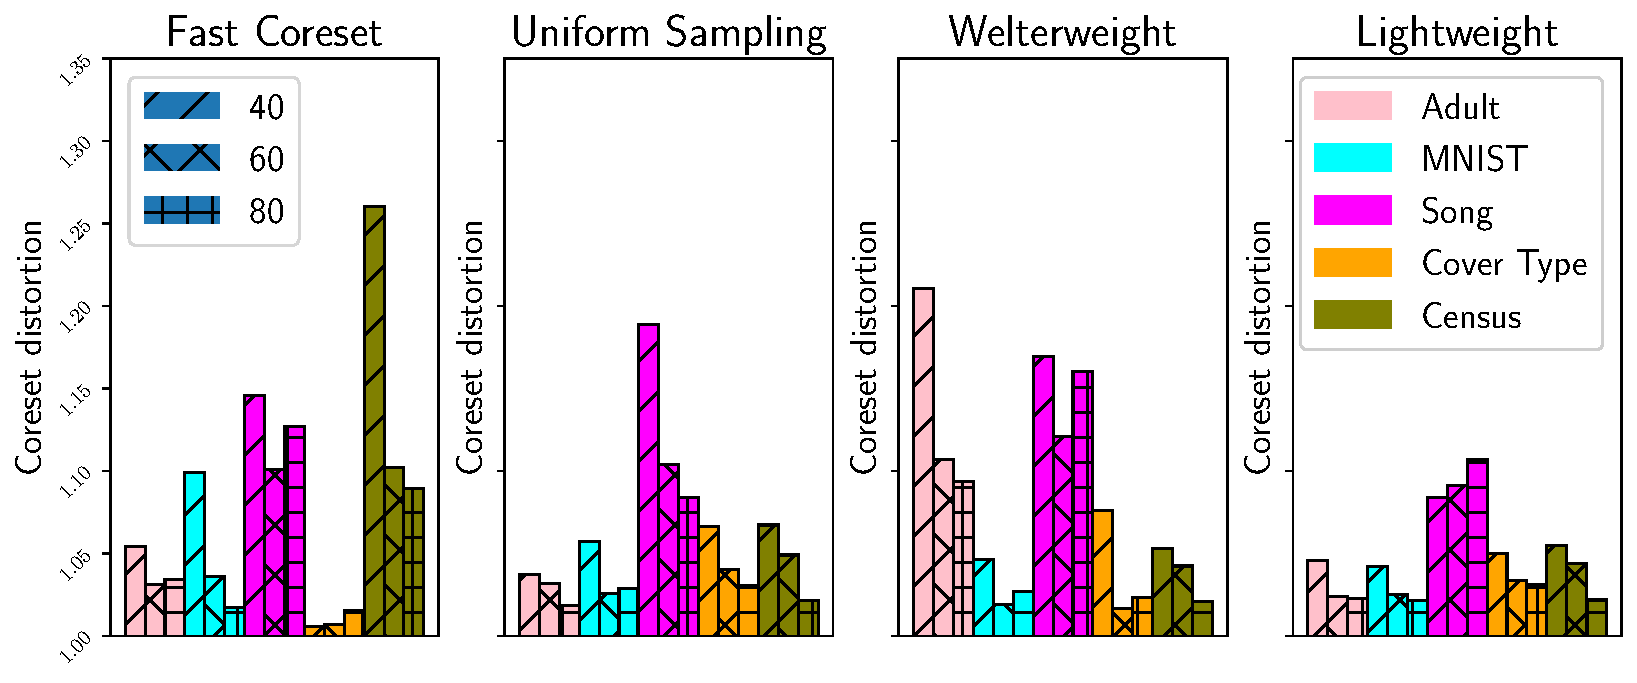
\includegraphics[width=\linewidth]{images/distortion_real_data} \\
    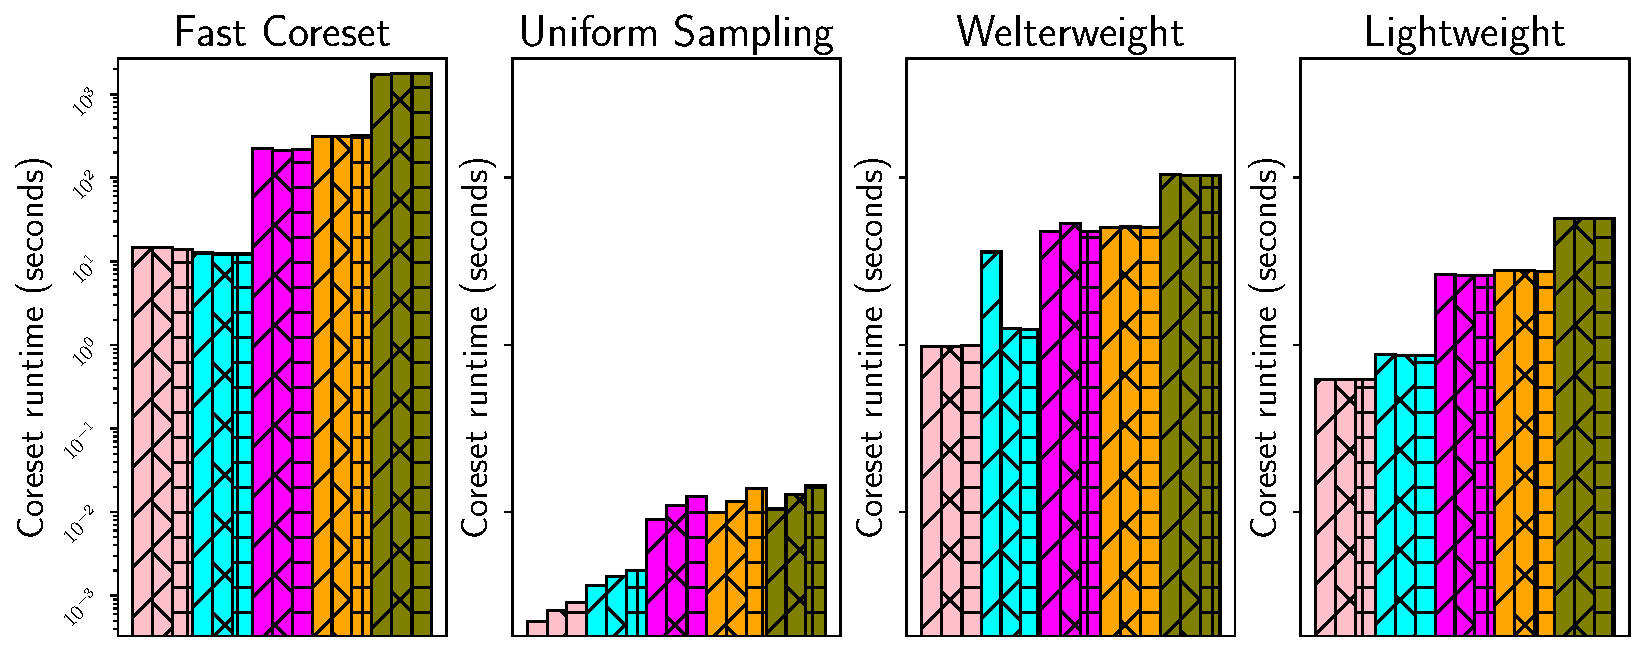
\includegraphics[width=\linewidth]{images/runtime_real_data}
\end{tabular}

\caption{\emph{Top}: The effect of the $m$-scalar on coreset distortion for real-world datasets. This is a visualization of the data in
Table~\ref{tbl:distortion}.  \emph{Bottom}: The effect of the $m$-scalar on the algorithm runtime for real-world datasets. All values are the mean over 5 runs.
The three bars represent samples of size $m=40k, 60k, 80k$.}

\label{fig:coreset_size_on_quality}
\end{figure}

